\documentclass[
	% -- opções da classe memoir --
	12pt,				% tamanho da fonte
	openright,			% capítulos começam em pág ímpar (insere página vazia caso preciso)
	oneside,			% para impressão em verso e anverso. Oposto a oneside
	a4paper,			% tamanho do papel. 
	% -- opções da classe abntex2 --
	%chapter=TITLE,		% títulos de capítulos convertidos em letras maiúsculas
	%section=TITLE,		% títulos de seções convertidos em letras maiúsculas
	%subsection=TITLE,	% títulos de subseções convertidos em letras maiúsculas
	%subsubsection=TITLE,% títulos de subsubseções convertidos em letras maiúsculas
	% -- opções do pacote babel --
	english,			% idioma adicional para hifenização
	french,				% idioma adicional para hifenização
	spanish,			% idioma adicional para hifenização
	brazil				% o último idioma é o principal do documento
	]{abntex2}


% --- 
% CONFIGURAÇÕES DE PACOTES
% --- 
% ---
% Pacotes básicos 
% ---
\usepackage{lmodern}			% Usa a fonte Latin Modern			
\usepackage[T1]{fontenc}		% Selecao de codigos de fonte.
\usepackage[utf8]{inputenc}		% Codificacao do documento (conversão automática dos acentos)
\usepackage{lastpage}			% Usado pela Ficha catalográfica
\usepackage{indentfirst}		% Indenta o primeiro parágrafo de cada seção.
\usepackage{color}				% Controle das cores
\usepackage{graphicx}			% Inclusão de gráficos
\usepackage{microtype} 			% para melhorias de justificação
\usepackage{ufc-abntex2}
% ---
		
% ---
% Pacotes adicionais, usados apenas no âmbito do Modelo Canônico do abnteX2
% ---
\usepackage{lipsum}				% para geração de dummy text
% ---

% ---
% Pacotes de citações
% ---
\usepackage[brazilian,hyperpageref]{backref}	 % Paginas com as citações na bibl
\usepackage[alf]{abntex2cite}	% Citações padrão ABNT

% ---
% Configurações do pacote backref
% Usado sem a opção hyperpageref de backref
\renewcommand{\backrefpagesname}{Citado na(s) página(s):~}
% Texto padrão antes do número das páginas
\renewcommand{\backref}{}
% Define os textos da citação
\renewcommand*{\backrefalt}[4]{
	\ifcase #1 %
		Nenhuma citação no texto.%
	\or
		Citado na página #2.%
	\else
		Citado #1 vezes nas páginas #2.%
	\fi}%
% ---

% ---
% Configurações de aparência do PDF final

% alterando o aspecto da cor azul
\definecolor{blue}{RGB}{41,5,195}

% informações do PDF
\makeatletter
\hypersetup{
     	%pagebackref=true,
		pdftitle={\@title}, 
		pdfauthor={\@author},
    	pdfsubject={\imprimirpreambulo},
	    pdfcreator={LaTeX with abnTeX2},
		pdfkeywords={abnt}{latex}{abntex}{abntex2}{trabalho acadêmico}, 
		colorlinks=true,       		% false: boxed links; true: colored links
    	linkcolor=blue,          	% color of internal links
    	citecolor=blue,        		% color of links to bibliography
    	filecolor=magenta,      		% color of file links
		urlcolor=blue,
		bookmarksdepth=4
}
\makeatother
% --- 

% --- 
% Espaçamentos entre linhas e parágrafos 
% --- 

% O tamanho do parágrafo é dado por:
\setlength{\parindent}{1.3cm}

% Controle do espaçamento entre um parágrafo e outro:
\setlength{\parskip}{0.2cm}  % tente também \onelineskip

% ---
% compila o indice
% ---
\makeindex
% ---


% Preambulo (Editar para mudar as variaveis do documento)
%
% Documento: Preâmbulo
%

\instituicao{Universidade Estadual do Sudoeste da Bahia}
\sigla{UESB}
\campus{Campus de Vitória da Conquista}
\local{Vitória da Conquista, Bahia}
\curso{Curso de Ciência da Computação}
\autor{Matheus Coqueiro Andrade}
\titulo{Estudo de caso sobre a utilização da Tecnologia da Informação Verde na Universidade Estadual do Sudoeste da Bahia}
%\subtitulo{Um estudo e aplicação}
\data{2018}
%\grau{Bacharel}
\dataapresentacao{29/06/2018}

%Dados Orientador
\orientador{Gidevaldo Novais Dos Santos}
\instOrientador{Universidade Estadual do Sudoeste da Bahia}
\departamentoorientador{Campus Vitória da Conquista}
\titulacaoorientador{Prof. Me.}

%Dados Coorientador
%\coorientador{Debra Morgan}
%\instCoorientador{Universidade Federal de Alagoas}
%\departamentocoorientador{Campus Arapiraca}
%\titulacaocoorientador{Prof. Me.}

%Dados Examinador 1
\nomeexamum{Helio Lopes Dos Santos}
\instexamum{Universidade Estadual do Sudoeste da Bahia}
\departamentoexamum{Campus Vitória da Conquista}
\titulacaoexamum{Prof. Dr.}

%Dados Examinador 2
\nomeexamdois{Roque Mendes Prado Trindade}
\instexamdois{Universidade Estadual do Sudoeste da Bahia}
\departamentoexamdois{Campus Vitória da Conquista}
\titulacaoexamdois{Prof. Dr.}

\tipotrabalho{Trabalho de Conclusão de Curso (Monografia)}
\preambulo{Trabalho de Conclusão de Curso apresentado como  requisito  parcial  para  obtenção  do grau de Bacharel em Ciência da Computação da  \imprimirinstituicao - \imprimirsigla, \imprimircampus.}


\begin{document}
\frenchspacing 

% ----------------------------------------------------------
% ELEMENTOS PRÉ-TEXTUAIS
% ----------------------------------------------------------
% \pretextual
% Capa
\imprimircapa
% Folha de rosto (* indica que haverá a ficha bibliográfica)
\imprimirfolhaderosto*

% Ficha Bibliográfica
% ---
% Inserir a ficha bibliografica
% ---

% Isto é um exemplo de Ficha Catalográfica, ou ``Dados internacionais de
% catalogação-na-publicação''. Você pode utilizar este modelo como referência. 
% Porém, provavelmente a biblioteca da sua universidade lhe fornecerá um PDF
% com a ficha catalográfica definitiva após a defesa do trabalho. Quando estiver
% com o documento, salve-o como PDF no diretório do seu projeto e substitua todo
% o conteúdo de implementação deste arquivo pelo comando abaixo:
%
% \begin{fichacatalografica}
%     \includepdf{fig_ficha_catalografica.pdf}
% \end{fichacatalografica}
\begin{fichacatalografica}
	\vspace*{\fill}					% Posição vertical
	\hrule							% Linha horizontal
	\begin{center}					% Minipage Centralizado
	\begin{minipage}[c]{12.5cm}		% Largura
	
	\imprimirautor
	
	\hspace{0.5cm} \imprimirtitulo  / \imprimirautor. --
	\imprimirlocal, \imprimirdata.
	
	\hspace{0.5cm} \pageref{LastPage} p. : il. (algumas color.) ; 30 cm.\\
	
	\hspace{0.5cm} \imprimirorientadorRotulo~\imprimirorientador\\
	
	\hspace{0.5cm}
	\parbox[t]{\textwidth}{\imprimirtipotrabalho~--~\imprimirinstituicao
	\par
	\imprimircampus
	\par
	Curso de \imprimircurso,
	\imprimirdata.}\\
	
	\hspace{0.5cm}
		1. TI Verde.
		2. Sustentabilidade.
		I. \imprimirorientador.
		II. \imprimirinstituicao.
		III. \imprimircurso.
		IV. \imprimirtitulo\\ 			
	
	\hspace{8.75cm} CDU 02:141:005.7\\
	
	\end{minipage}
	\end{center}
	\hrule
\end{fichacatalografica}
% ---

% Errata
%\include{editaveis/errata}

% Folha de Aprovação
% ---
% Inserir folha de aprovação
% ---

% Isto é um exemplo de Folha de aprovação, elemento obrigatório da NBR
% 14724/2011 (seção 4.2.1.3). Você pode utilizar este modelo até a aprovação
% do trabalho. Após isso, substitua todo o conteúdo deste arquivo por uma
% imagem da página assinada pela banca com o comando abaixo:
%
% \includepdf{folhadeaprovacao_final.pdf}
%
\begin{folhadeaprovacao}

  \begin{center}
    {\bfseries\Large\imprimirautor}
    \vspace{1cm}

    \begin{center}
      \bfseries\Large\imprimirtitulo
    \end{center}

    \vspace{2cm}
    \begin{minipage}{\textwidth}
        \imprimirpreambulo
        \\ \\ \\
        Aprovada em: \imprimirdataapresentacao
    \end{minipage}%
     
    \vspace{2cm}
	\textbf{BANCA EXAMINADORA}
	
	\vspace*{1.2 cm}%Espaçamento entre linhas
    \rule{9 cm}{.1 mm}\\
    {\imprimirtitulacaoorientador}{ }{\imprimirorientador}\\
    {\imprimirinstOrientador}\\
    {\imprimirdepartamentoorientador}\\
    Orientador\\

    \vspace*{1.1 cm}%Espaçamento entre linhas
    \rule{9 cm}{.1 mm}\\
    \imprimirtitulacaoexamum{ }\imprimirnomeexamum\\
    \imprimirinstexamum\\
    \imprimirdepartamentoexamum\\
    Examinador\\

    \vspace*{1.1 cm}%Espaçamento entre linhas
    \rule{9 cm}{.1 mm}\\				
    				
    \imprimirtitulacaoexamdois{ }\imprimirnomeexamdois\\
    \imprimirinstexamdois\\
    \imprimirdepartamentoexamdois\\
    Examinador
    \vspace*{1.3 cm}%Espaçamento entre linhas
   \end{center}
  
\end{folhadeaprovacao}
% ---

%\imprimirfolhadeaprovacao

% Dedicatória
% ---
% Dedicatória
% ---

\begin{dedicatoria}
   \vspace*{\fill}
   	\begin{flushright}
   \noindent
   Este trabalho é dedicado aos meus pais, que foram o meu porto seguro e me deram todo o suporte possível para que eu chegasse até o final.
   	\end{flushright}
\end{dedicatoria}
% ---

% Agradecimentos
% ---
% Agradecimentos
% ---
\begin{agradecimentos}
  %
  %   Editar ainda!!!
  %

  Aos meus pais. 

  Agradeço à minha namorada Rafaela Oliveira.

  Amigos Especiais (Maioli, Yuri e Wanderson).

  Colegas de turma, curso em especial ao Lindalva.

  Aos professores, em especial ao professor roque, marco antônio e alzira.

  À celina.

  Aos meus amigos que ficaram pelo meio do caminho, Iury Simmont, Jade Dias, Laherce, Matheus Couto, Pedro Barros e Raveni, vocês foram mais que meus amigos, foram a minha família. 
\end{agradecimentos}
% ---

% Epígrafe
% ---
% Epígrafe
% ---
\begin{epigrafe}
    \vspace*{\fill}
	\begin{flushright}
		\textit{``Para ter sucesso neste mundo não basta ser \\
		estúpido, é preciso também ter boas maneiras\\
		(Voltaire)}
	\end{flushright}
\end{epigrafe}
% ---

% Resumo
% resumo em português
\setlength{\absparsep}{18pt} % ajusta o espaçamento dos parágrafos do resumo
\begin{resumo}
 Segundo a NBR6028:2003, o resumo deve ressaltar o
 objetivo, o método, os resultados e as conclusões do documento. A ordem e a extensão
 destes itens dependem do tipo de resumo (informativo ou indicativo) e do
 tratamento que cada item recebe no documento original. O resumo deve ser
 precedido da referência do documento, com exceção do resumo inserido no
 próprio documento. (\ldots) As palavras-chave devem figurar logo abaixo do
 resumo, antecedidas da expressão Palavras-chave:, separadas entre si por
 ponto e finalizadas também por ponto.

 \textbf{Palavras-chaves}: latex. abntex. editoração de texto.
\end{resumo}

% Abstract
% resumo em inglês
\begin{resumo}[Abstract]
 \begin{otherlanguage*}{english}
 

   \vspace{\onelineskip}
 
   \noindent 
   \textbf{Key-words}: latex. abntex. text editoration.
 \end{otherlanguage*}
\end{resumo}

% Lista de ilustrações
\pdfbookmark[0]{\listfigurename}{lof}
\listoffigures*
\cleardoublepage

% Lista de tabelas
\pdfbookmark[0]{\listtablename}{lot}
\listoftables*
\cleardoublepage

% Abreviaturas e Siglas
% Lista de abreviaturas e siglas
% ---
\begin{siglas}
    \item[AGESPI]   Assessoria na Gestão de Projetos e Convênios Institucionais
    \item[AIIM]	    \textit{Association for Information and Image Management}
    \item[APG]	    Assessoria de Gestão de Pessoas
    \item[CEUAS]	Centro Universitário de Atenção à Saúde
    \item[CRM]	    \textit{Costumer Relationship Management}
    \item[DLL]	    \textit{Dynamic Link Library}
    \item[EAI]	    \textit{Enterprise Apliccation Integration}
    \item[EPA]	    \textit{Environmental Protection Agency}
    \item[ERM]  	\textit{Enterprise Report Management}
    \item[FAINOR]	Faculdade Independente do Nordeste
    \item[FTC]  	Faculdade de Tecnologia e Ciências
    \item[ERP]	    \textit{Enterprise Resource Planning}
    \item[GED]	    Gestão Eletrônica de Documentos
    \item[IFBA]	    Instituto Federal da Bahia
    \item[PCF]	    Posto de Cadastro de Fornecedores
    \item[PDM]	    \textit{Product Data Management}
    \item[PEN]	    Processo Eletrônico Nacional
    \item[PID]  	Plano de Desenvolvimento Institucional
    \item[Procel]	Programa Nacional de Conservação de Energia Elétrica
    \item[REEE]	    Resíduos de Equipamentos Eletroeletrônicos
    \item[RH]   	Recursos Humanos
    \item[RoHS]	    \textit{Restriction of Certain Hazardous Substances}
    \item[RSE]  	Responsabilidade Social Empresarial
    \item[SEI]  	Sistema Eletrônico de Informação
    \item[SGA]  	Sistema de Gestão Ambiental
    \item[SIF]  	Setor de Informações Funcionais
    \item[TI]   	Tecnologia da Informação
    \item[TI Verde]	Tecnologia da Informação Verde
    \item[TIC]  	Tecnologia da Informação e Comunicação
    \item[TRF4]	    Tribunal Regional Federal da 4a Região
    \item[UESB]	    Universidade Estadual do Sudoeste da Bahia
    \item[UFBA]	    Universidade Federal da Bahia
    \item[UINFOR]	Unidade Organizacional de Informática
    \item[VDI]	    \textit{Virtual Desktop Infrastructure}
    \item[WEEE]	    \textit{Waste Electrical and Electronic Equipment Directive}
    
    

\end{siglas}
% ---

% Símbolos
%%Lista de símbolos
% ---
\begin{simbolos}
  \item[$ \Gamma $] Letra grega Gama
  \item[$ \Lambda $] Lambda
  \item[$ \zeta $] Letra grega minúscula zeta
  \item[$ \in $] Pertence
\end{simbolos}
% ---

% Sumário
\pdfbookmark[0]{\contentsname}{toc}
\tableofcontents*
\cleardoublepage

% ----------------------------------------------------------
% ELEMENTOS TEXTUAIS
% ----------------------------------------------------------
\textual

% ----------------------------------------------------------
% PARTE I
% ----------------------------------------------------------
\part{Preparação da pesquisa}

%
% Documento: Introdução
%

\chapter{Introdução}\label{chap:introducao}

Em tempos de globalização econômica e de comunicação, é de suma importância pensar nas gerações futuras. Segundo o relatório de \citeonline{brundtland1987report}, o ``desenvolvimento sustentável é o desenvolvimento que satisfaz as necessidades do presente sem comprometer a capacidade das futuras gerações satisfazerem suas próprias necessidade''. 

Para \citeonline{hart1995natural}, o desenvolvimento sustentável está relacionado com o crescimento sem prejuízos aos recursos naturais utilizados, onde a preocupação com os fatores ambientais são prioridade. 

Para as empresas e instituições, fica clara a necessidade de se adotar estratégias e modelos para se adequar ao desenvolvimento sustentável, a Tecnologia da Informação Verde (TI Verde).


%essa frase ficou longa pra caralho eu achei. Eu quebraria depois do "TI verde" e colocaria nessa pegada:
%(...) sobre a importância de se implementar modelos de Tecnologia da Informação Verde. Outra justificativa é o alto consumo de energia nesse tipo de instituição, que pode ser atacado por meio de uma série de vantagens da TI Verde, pois já existem dispositivos (...)
\section{Justificativa}

Hoje a Universidade Estadual do Sudoeste da Bahia (UESB) é a maior instituição de ensino da Mesorregião do Centro-Sul Baiano. Ela possui grande influência na comunidade local, tendo a responsabilidade social de implementar práticas sustentáveis e possuir um Sistema de Gestão Ambiental, tornando-se referência de sustentabilidade no âmbito tecnológico, criando uma iniciativa nesta área que atualmente é pouca explorada. Com isso, existe a chance de se conscientizar os gestores das demais instituições de ensino e empresas, sobre a importância, vantagens e ganhos, de se aplicar práticas verdes. 

\section{Questão da pesquisa}
Nos dias atuais, existe uma necessidade das organizações pensarem em maneiras de otimizar o uso das tecnologias, de modo que contribuam com a sustentabilidade e o desenvolvimento sustentável, minimizando os riscos e impactos ambientais e atendendo às dimensões da sustentabilidade (ambiental, social e econômica). Neste contexto, existem as seguintes questões que esta pesquisa tentará resolver:
\begin{itemize}
    \item Como a Tecnologia da Informação Verde é utilizada na Universidade Estadual do Sudoeste da Bahia, campus de Vitória da Conquista?
    \item A Universidade Estadual do Sudoeste da Bahia utiliza a Tecnologia da Informação Verde de maneira correta?
    \item Como a Tecnologia da Informação Verde pode ser aplicada na Universidade Estadual do Sudoeste da Bahia, visando ter uma redução no consumo de energia, geração de Resíduos de Equipamentos Eletroeletrônicos e gasto com a manutenção?
\end{itemize}

\section{Objetivo geral}
Apresentar os benefícios de utilizar práticas da Tecnologia da Informação Verde, contribuindo para a diminuição dos riscos ou dos impactos ambientais causados pela má utilização da tecnologia, além da redução dos gastos. 

\section{Objetivos específicos}
Realizar um estudo sobre a TI Verde, verificando as soluções que visam o melhor uso da tecnologia da informação, garantindo à redução dos impactos ambientais.
 
Analisar a utilização da TI Verde na Unidade Organizacional de Informática da UESB, campus de Vitória da Conquista.  

Propor novas soluções baseadas nas práticas da TI Verde, apresentando os ganhos que a instituição terá por implementar essas soluções.


\section{Metodologia}

\subsection{Tipo de pesquisa}
A modalidade desta pesquisa é de campo e bibliográfica. Quanto aos objetivos é do tipo exploratória e descritiva, e quanto à forma de abordagem é qualitativa, com aplicação de entrevista estruturada, entrevista semiestruturada e de um questionário.

\subsection{Campo de pesquisa}

A entrevista semiestruturada e o questionário foram aplicadas com o diretor da Unidade Organizacional de Informática da UESB (UINFOR). A entrevista foi realizada no dia 15 de Junho de 2018, utilizando o aplicativo de mensagens instantâneas \textit{WhatsApp Messenger}, já o questionário foi aplicado no dia 17 de Abril de 2018, utilizando o editor de texto online Google Documentos. Também foi realizado a leitura do Roteiro de Diagnóstico Setorial, disponibilizado pelo entrevistado, que descreve todas as funções, atribuições, atividades, estruturas e processos da UINFOR, além do Plano de Desenvolvimento Institucional (PID) 2013-2017$^{[}$\footnote{PID 2013-2017, Disponível em: \url{http://www.uesb.br/pdi/arquivos/PDI_Final.pdf}.  Acessado em 16 de junho de 2018}$^{]}$ que contém diversas informações sobre a UESB.

A entrevista estruturada foi aplicada com o analista e desenvolvedor do projeto de Gestão Eletrônica de Documentos (GED), do Setor de Informações Funcionais (SIF). A entrevista foi realizada no dia 14 de Junho de 2018, utilizando o editor de texto online Google Documentos e o aplicativo de mensagens instantâneas \textit{WhatsApp Messenger}.

\subsection{Coleta de dados}
A obtenção de dados relacionados ao estudo de caso foi realizada mediante aplicação de um questionário (Apêndice A), uma entrevista semiestruturada (Apêndice B) e uma entrevista estruturada (Apêndice C). As perguntas das entrevistas foram elaboradas pelo pesquisador a partir do conhecimento obtido pelo referencial teórico, se baseando em alguns trabalhos estudados. Foram contemplados tópicos considerados de relevância para o tema pelo pesquisador, a fim de coletar dados no que se refere à utilização da TI verde pela instituição, de modo que se possa medir o grau de adequação com base nas respostas encontradas.

O questionário aplicado foi extraído de \citeonline{lunardi2014desenvolvimento}, e serve para avaliar o grau de utilização da TI Verde pelas organizações. Ele é dividido em 5 fatores, apresentados a seguir: 
\begin{itemize}
    \item  \textbf{Consciência socioambiental:} Avalia se a organização está consciente da necessidade de abordar as questões ambientas de forma mais proativa;
    \item \textbf{Ações sustentáveis:} Avalia se a organização implementa iniciativas para tornar os processos o mais sustentável possível;
    \item \textbf{\textit{Expertise} ambiental:} Avalia se a organização se submete a experimentar, atualizar e buscar novas abordagens, informações e conhecimentos a fim de aplicar estratégias sustentáveis na área de Tecnologia da Informação;
    \item \textbf{Monitoramento:} Avalia se a organização gerencia as atividades e medidas de Tecnologia da Informação voltadas à redução do consumo de recursos e dos danos ao meio ambiente;
    \item \textbf{Orientação ambiental:} Avalia se a organização está comprometida com a sustentabilidade e com o suporte às inovações ambientais.
\end{itemize}

As informações para o embasamento teórico foram coletadas através de fontes primárias como livros, artigos, monografias e leis sobre o referido tema, e fontes complementares, como sites da internet. 

Após a coleta de dados, foi identificada e medida à utilização da TI Verde, e propostas novas soluções para serem utilizadas pela instituição.

\subsection{Estrutura de desenvolvimento}
A estrutura de desenvolvimento do projeto de pesquisa foi dividido nas seguintes etapas:

\begin{itemize}
  \item Realizar um estudo sobre a TI Verde;
  \item Pesquisar e conhecer como a TI Verde é utilizada atualmente na UESB, em Vitória da Conquista;
  \item Identificar as maiores necessidades e problemas relacionados à Tecnologia da Informação que a UESB enfrenta;
  \item Propor soluções baseadas nas práticas de TI Verde;
  \item Apresentar uma conclusão sobre a utilização de TI Verde na UESB.
\end{itemize}


\section{Estrutura do trabalho}

% ----------------------------------------------------------
% PARTE II
% ----------------------------------------------------------
\part{Referenciais teóricos}

%
% Documento: Tecnologia de Informação Verde
%

\chapter{Tecnologia da Informação Verde}

\section{Informação}

De acordo com \citeonline{pinheiro2004informaccao}, a informação é dependente de um contexto (científico, tecnológico, industrial, artístico, cultural, entre outros). Segundo \citeonline[p. 17]{aguilar2009tecnologia}, a informação corresponde a grupos de dados classificados e organizados, que tenham valor para que uma pessoa ou empresa consiga utilizar para seu benefício. Na vida real ou empresarial, dispor de informação é um fator determinante para o sucesso e seu mal-uso pode trazer prejuízos astronômicos. Para ajudar a resolver esses problemas existe o que chamam de Tecnologia da Informação (TI).

\section{Tecnologia da Informação}

A evolução humana tem ligação direta com o avanço da tecnologia, bem como o contrário. Um é inerente ao outro e isso é indiscutível quando observamos as várias mudanças nos instrumentos, que se tornaram mais funcionais, acompanhando a evolução do homem, tanto na anatomia de seu corpo, principalmente de sua mão, quanto em seu cérebro. \cite[p. 107-111]{acevedo1998ciencia}. Ela foi desenvolvida para satisfazer as necessidades humanas e já existia antes dos homens e dos conhecimentos científicos e mesmo assim foi capaz de criar estruturas e instrumentos complexos. \cite{acevedo1998ciencia, veraszto2004projeto}. 

Para \citeonline[p. 2]{de1996tecnologia}, a tecnologia pode ser definida como conjunto de conhecimentos, de sua maioria científicos, que são aplicados em determinados ramos de atividades. Podendo ser considerada uma ciência que trata da técnica.

A TI é um dos campos da tecnologia que tomou força no século XX. Surgiu como um meio para melhorar os processos de criação e desenvolvimento \cite[p. 2]{de1996tecnologia}, e atualmente é um forte indicador de melhoria na performance e produtividade \cite[p. 2]{lunardi2001efeitos}, além de ter grande relevância na continuação de esforços das empresas para tornarem os seus processos mais ágeis e produtivos \cite{shaw1997information}. Seu grande papel é o gerenciamento de informações, mas nem sempre esse gerenciamento se dá de forma agradável para o meio ambiente \cite[p. 6-7]{silva2011}. Para solucionar os problemas e amenizar os impactos decorrentes da tecnologia de informação pesquisadores desenvolveram as práticas da Tecnologia da Informação Verde.

\section{Tecnologia da Informação Verde}

O grande avanço tecnológico dos últimos anos, acompanhado da obsolescência programada dos produtos e do consumo desenfreado com consequente produção em grande escala resultam em grandes riscos para o meio ambiente. O descarte inadequado do lixo eletroeletrônico tem grande impacto ambiental e traz sérios riscos à saúde humana, uma das causas é a contaminação de solos e águas com minérios pesados. Há também o grande gasto de energia, uma vez que o número de aparelhos eletrônicos vem crescendo em empresas e indústrias além de vários serviços que são utilizados 24h horas por dia ou são atualizados sempre, impedindo seu desligamento durante a noite ou fins de semana.

Segundo \citeonline[p. 2]{laurindo2000estudo}, a tecnologia “não só sustenta as estratégias de negócio existentes, mas também permite que se viabilizem novas estratégias empresariais”. Uma dessas novas estratégias surgiu com a busca pela redução dos impactos ambientais e a possível reversão de danos causados, o que resultou no estabelecimento de práticas sustentáveis na área de TI, que juntas são conhecidas como TI Verde. \cite{aguilar2009tecnologia}.

A TI Verde vem do conceito de ecoeficiência, e teve origem na década de 80, e se consiste do uso eficiente dos recursos naturais, e na última década vem sendo utilizado com frequência nos setores de TI. \cite{ferreira2009tiverde}. Atualmente, a TI Verde pode ser definida como um conceito que as empresas de tecnologia criaram para agregar o uso de recursos tecnológicos e políticas que minimizem cada vez mais as agressões ao meio ambiente. \cite{briefing2008preciso}.

\begin{citacao}
A TI Verde é o estudo e a prática de projetar, fabricar,
usar e descartar computadores, servidores e subsistemas associados (monitores, impressoras, dispositivos de armazenamento e de rede e sistemas de comunicação), de forma eficiente e eficaz, com o mínimo de impacto para o meio ambiente, lutando para atingir a viabilidade econômica e melhorar o uso e o desempenho dos sistemas e respeitando as responsabilidades sociais e éticas. \cite{lunardi2014desenvolvimento}.
\end{citacao} 

Para \citeonline[p. 36]{aguilar2009tecnologia}, a economia de energia e corte de gastos sempre foram as grandes preocupações das empresas. Essa preocupação se torna ainda maior na área de TI, pois os \textit{datacenters} geralmente costumam figurar como a maior porcentagem dos gastos de energia elétrica de uma companhia, já que em um banco, por exemplo, a energia que a TI utiliza pode superar a metade de todo consumo.  

Além da preocupação com o meio ambiente, várias dessas práticas têm um impacto econômico positivo, o que contribui para sua ampla adoção, já que a busca pelo aumento da produtividade passa pela redução de gastos e tem influência direta da utilização de recursos básicos, como água, energia e matérias primas.

\section{Tecnologia da Informação Verde nas organizações}

Para \citeonline{kraemer2005responsabilidade} o fator ambiental vem mostrando a necessidade de adaptação das organizações e consequentemente direcionando novos caminhos na sua expansão. As organizações precisam alterar seus paradigmas, mudando sua visão empresarial, objetivos, estratégias de investimentos e de marketing, se adaptando à nova realidade do mercado global e ecologicamente correto.

\begin{citacao}
As empresas têm um papel extremamente relevante. Através de uma prática empresarial sustentável, provocando mudança de valores e de orientação em seus sistemas operacionais, estarão engajadas à ideia de desenvolvimento sustentável e preservação do meio ambiente \cite[p. 3]{kraemer2005responsabilidade}. 
\end{citacao}

Os desequilíbrios sócio-ambientais são o resultado do velho paradigma cartesiano e mecanicista, com sua visão fragmentada do mundo \cite[p. 28]{almeida2002bom}. Este paradigma é meramente capitalista e visa o lucro máximo, fazendo com que o meio ambiente seja apenas um bem privado, no que se refere à produção e descarte dos seus resíduos. Este modelo não é sustentável ao longo do tempo, pois ficou claro que os recursos naturais são esgotáveis e, portanto, finitos, se mal utilizados \cite{kraemer2005responsabilidade}.

A \autoref{tab:cartesiano-sustentabilidade} apresenta uma comparação do paradigma atual com o paradigma sustentável.

\begin{table}[htb]	
    \ABNTEXfontereduzida
	\Caption{\label{tab:cartesiano-sustentabilidade} Paradigma cartesiano \textit{versus} paradigma da sustentabilidade.}
	\UECEtab{}{
		\begin{tabular}{p{7cm}p{8cm}}
			\toprule
    		\textbf{Cartesiano} & \textbf{Sustentável} \\
			\midrule \midrule
				Reducionista, mecanicista, tecnocêntrico  & Orgânico, holístico, participativo \\
				Fatos e valores não relacionados & Fatos e valores fortemente relacionados \\
				Preceitos éticos desconectados das práticas cotidianas & Ética integrada ao cotidiano \\
				Separação entre o objetivo e o subjetivo & Interação entre o objetivo e o subjetivo \\
				Seres humanos e ecossistemas separados, em uma relação de dominação & Seres humanos inseparáveis dos ecossistemas, em uma relação de sinergia \\
				Conhecimento compartimentado e empírico  & Conhecimento indivisível, empírico e intuitivo \\
				Relação linear de causa e efeito & Relação não-linear de causa e efeito \\
				Natureza entendida como descontínua, o todo formado pela soma das partes  & Natureza entendida como um conjunto de sistemas inter-relacionados, o todo maior que a soma das partes \\
				Bem-estar avaliado por relação de poder (dinheiro, influência, recursos)  & Bem-estar avaliado pela qualidade das inter-relações entre os sistemas ambientais e sociais \\
				Ênfase na quantidade (renda per capita) & Ênfase na qualidade (qualidade de vida) \\
				Análise & Síntese \\
				Centralização de poder & Descentralização de poder \\
				Especialização & Transdisciplinaridade \\
				Ênfase na competição & Ênfase na cooperação \\
				Pouco ou nenhum limite tecnológico  & Limite tecnológico definido pela sustentabilidade \\
			\bottomrule
		\end{tabular}
	}{
		\Fonte{\citeonline{almeida2002bom}}
    }
\end{table}

\subsection{Responsabilidade Social}

O Governo vem pressionando cada vez mais as organizações para que desenvolvam práticas para reduzir seus impactos ambientais e sociais. Recentemente, houveram grandes progressos quanto à conscientização sobre a responsabilidade social e maior compreensão dos desafios da sustentabilidade \cite{kraemer2005responsabilidade}.

A Responsabilidade Social Empresarial (RSE) pode ser conceituada através da integração das preocupações sociais e ambientais em suas operações e interação com todas as partes interessadas. É caraterizada pela sua adoção voluntária, para além das prescrições legais. Este conceito é associado com o de desenvolvimento sustentável, onde as organizações integram em suas operações o impacto econômico, social e ambiental \cite{biorumo}.  

A RSE conta com três fatores fundamentais: o planeta (preocupações ambientais), as pessoas (preocupações sociais) e a rentabilidade (preocupações econômicas), esta tridimensionalidade é definida pela expressão \textit{Triple Bottom Line}, apresentada na figura \autoref{fig_triple_bottom_line} \cite{biorumo}.


\begin{figure}[htb]
    \caption{\label{fig_triple_bottom_line}\textit{Triple Bottom Line}.}
    \begin{center}
        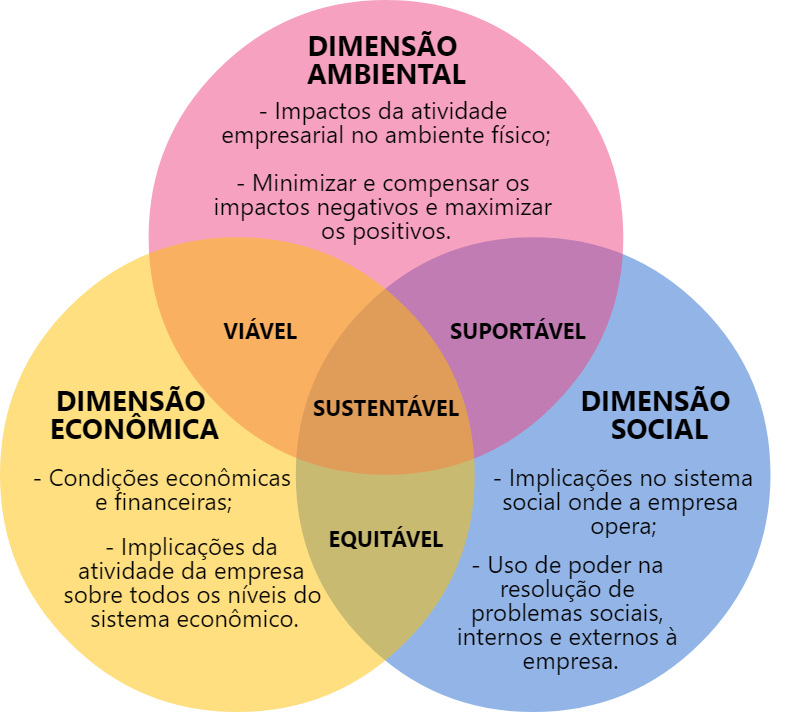
\includegraphics[scale=0.45]{imagens/triple-bottom-line.png}
    \end{center}
    \FonteFigura{Adaptado de \citeonline[p. 24]{biorumo}.}
\end{figure}

\subsection{Gestão Ambiental}

Alguma coisa...

\section{As práticas de TI Verde}

%As práticas de TI Verde, nos dias atuais, são utilizadas como estratégias de negócio na maior parte das grandes das empresas. Elas garantem lucros, bem-estar e reconhecimento da empresa, além de ajudar na proteção do meio ambiente, melhorando o futuro das próximas gerações, tornando-se imprescindível no dia a dia de qualquer empresa.%

A adoção de práticas sustentáveis é bem vista e traz maior reconhecimento para as organizações que as utilizam, pois, a sociedade atual se preocupa com a preservação do meio ambiente. \cite{abreu2012ti}. Essas práticas são aplicadas de acordo com cada perfil de organização. Nos dias atuais, é indispensável uma análise estrutural da empresa para identificar qual prática mais se adéqua a sua realidade. A implementação dessas práticas trará benefícios tanto para o meio ambiente, como também para a empresa. \cite{pinto2011estudo}.

Estas práticas envolvem ações diversas com o objetivo de economizar recursos e aumentar a durabilidade dos equipamentos usados.  São elas economia de energia, virtualização de servidores e \textit{desktop}, videoconferência, economia de papel e descarte, e reciclagem de REEE. Com o avanço tecnológico surgirão novas práticas de TI Verde para que o uso da TI se torne sustentável \cite[p. 8]{pinto2011estudo}.

\subsection{Os três níveis}

\citeonline{takahashi2009ti} e \citeonline[p. 7]{pinto2011estudo} classificam as práticas de TI Verde em três níveis:

\subsubsection{TI Verde Tático}

Nesse nível as práticas implementadas não modificam a infraestrutura nem interferem nas políticas internas do local, além de não gerarem custos adicionais. Abrangem mudanças ligadas à economia de recursos e tem como medidas o controle do uso excessivo de energia elétrica de uma organização. Alguns exemplos são o monitoramento automático do gasto de energia dos equipamentos, desligando-os quando estão em desuso, o uso de lâmpadas mais eficientes e a mudança na organização e disposição dos equipamentos para melhor circulação e consequente dissipação do calor, otimizando assim a temperatura das salas.

\subsubsection{TI Verde Estratégico}

Nesse nível as mudanças realizadas envolvem a convocação de uma auditoria da infraestrutura de TI e do seu uso relacionado ao meio ambiente e novos meios de produção de bens ou serviços são desenvolvidos e implementados de maneira ecológica. São criadas novas políticas internas e medidas de controle e descarte dos REEE. A adoção destas medidas geram um \textit{marketing} positivo, melhorando assim a imagem dessa organização diante da sociedade. Algumas práticas realizadas neste nível, diferentemente do anterior, geram um custo adicional devido a criação de uma nova rede elétrica visando uma maior eficiência energética e de sistemas computacionais que tenham um menor consumo elétrico, por meio da substituição dos equipamentos por outros mais econômicos e possíveis reformas estruturais.

\subsubsection{TI Verde a Fundo}

Esse nível é a integração dos níveis anteriores. É necessário a criação de um projeto de total modificação estrutural para maximizar a economia de energia e a sustentabilidade da organização. São realizadas grandes mudanças na infraestrutura que visam o otimizar o desempenho dos equipamentos e a padronização dos processos, como projetos de sistemas de refrigeração, iluminação e disposição de equipamentos, gerando um alto custo para a sua implementação.

\subsection{Virtualização}

A virtualização é uma técnica utilizada para emular um ambiente computacional sobre outro, ela é bastante popular na maioria das organizações, pois ela reduz aumento do número de maquinas físicas quando se tem uma diversidade de sistemas operacionais. As máquinas virtuais\footnote{Nome dado para ambientes computacionais simulados} podem ter múltiplas instâncias em um mesmo \textit{hardware} e incluem as bibliotecas do sistema operacional desejado, proporcionando um uso eficiente do seu poder de processamento e um alto grau de portabilidade. A redução de maquinas físicas implica na queda dos gastos da infraestrutura, como espaço, energia elétrica, cabeamento, refrigeração, suporte e manutenção de vários sistemas \cite[p. 174-175]{carissimi2008virtualizaccao}.

\citeonline[p. 193]{carissimi2008virtualizaccao} e \citeonline[p. 163-165]{neto2015ti} apresentam os seguintes métodos de virtualização oferecidos pela \textit{Microsoft}:
\begin{itemize}
    \item Virtualização de Servidor: as máquinas virtuais são criadas através de um software onde as mesmas emulam servidores, permitindo a execução dos seus sistemas operacionais de maneira simultânea. Dois ou mais servidores virtuais são emulados em um único servidor físico, otimizando o uso da memória, processamento e armazenamento (\autoref{fig_virt_serv});
    
    \begin{figure}[htb]
    	\caption{\label{fig_virt_serv}Virtualização de Servidores.}
    	\begin{center}
    	    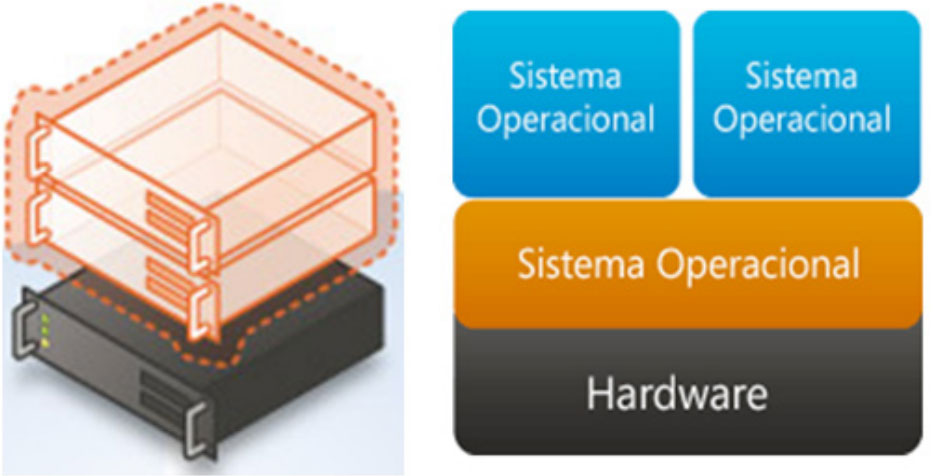
\includegraphics[scale=0.3]{imagens/virtualizacao-servidor.jpg}
    	\end{center}
    	\FonteFigura{\citeonline[p. 163]{neto2015ti}.}
    \end{figure}
    
    \item Virtualização de Estação de Trabalho ou VDI (\textit{Virtual Desktop Infrastructure} - Infraestrutura de estação de trabalho virtual): é utilizado para simular uma maquina virtual "inteira", permitindo o gerenciamento de estações de trabalho com maior eficiência atendendo as necessidades dos usuários. É utilizada para quando existe a necessidade de executar \textit{software} legado\footnote{Termo utilizado para sistemas computacionais que, apesar de serem bastante antigos, fornecem serviços essenciais.}, criar ambientes de testes e treinamento. Cada estação possui seu ambiente com sistema operacional e aplicações independentes. (\autoref{fig_vdi});
    
    \begin{figure}[htb]
    	\caption{\label{fig_vdi}Virtualização de Desktop.}
    	\begin{center}
    	    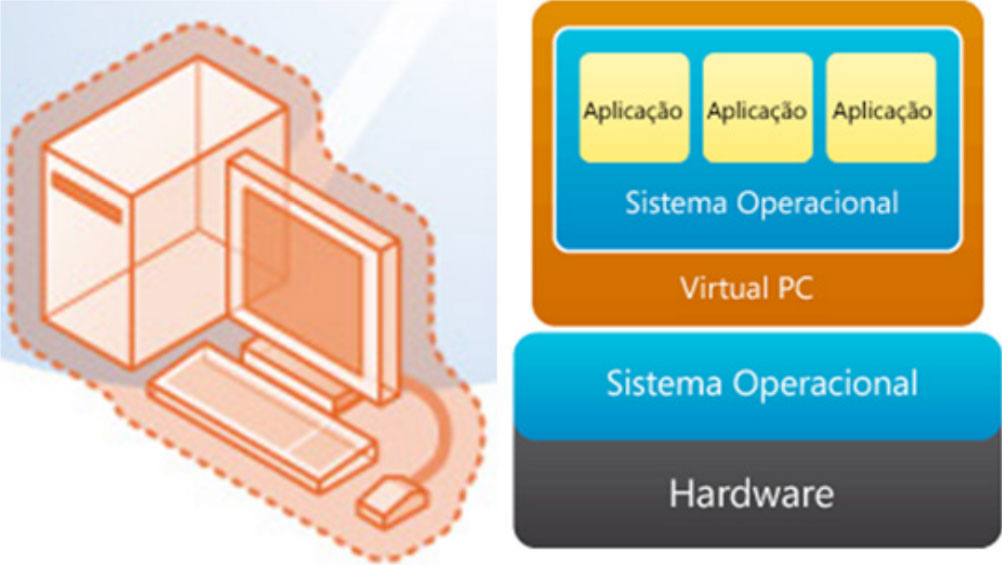
\includegraphics[scale=0.3]{imagens/vdi.jpg}
    	\end{center}
    	\FonteFigura{\citeonline[p. 164]{neto2015ti}.}
    \end{figure}
    
    \item Virtualização de Aplicações: tem como objetivo oferecer aplicações por demanda. A aplicação é alocada em um servidor virtual, que a executa dentro de um próprio ambiente, com isso o usuário não precisa instala-la em sua estação. Cada aplicação fica isolada umas das outras e do sistema operacional subjacente, permitindo ou não a interação e compartilhamento de componentes como dll's\footnote{sigla para \textit{Dynamic Link Library} e se trata de uma biblioteca dinâmica que contém dados que podem ser acessados por mais de um programa instalado no computador} e \textit{Drivers} (\autoref{fig_virt_apli});
    
    \begin{figure}[htb]
    	\caption{\label{fig_virt_apli}Virtualização de Aplicações.}
    	\begin{center}
    	    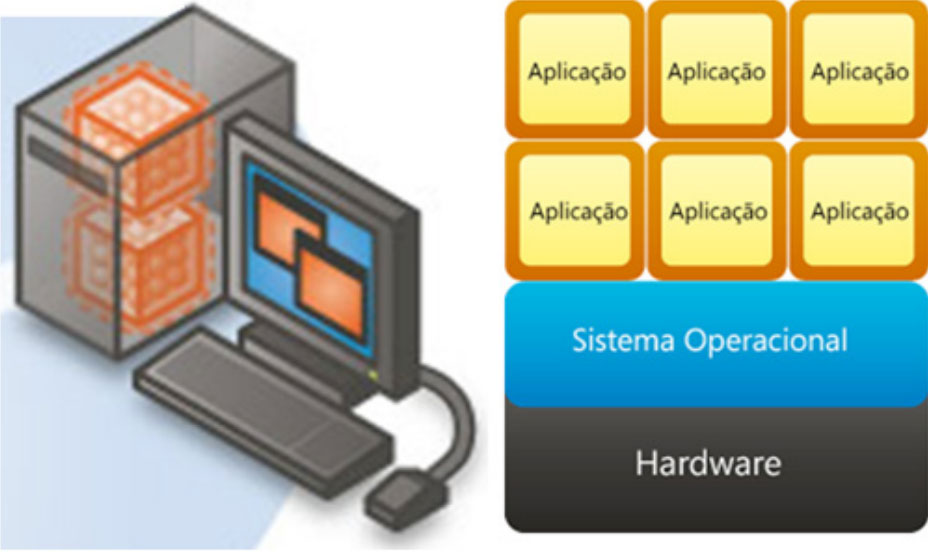
\includegraphics[scale=0.3]{imagens/virtualizacao-aplicacao.jpg}
    	\end{center}
    	\FonteFigura{\citeonline[p. 164]{neto2015ti}.}
    \end{figure} 
    
    \item Virtualização de Apresentação: consiste de um ambiente computacional para acesso à distância, permitindo que uma determinada aplicação seja executada em uma máquina, mas utilize recursos gráficos e de Entrada/Saída de outra e que vários usuários utilizem o sistema não interferindo uns com os outros (\autoref{fig_virt_apre});
    
    \begin{figure}[htb]
    	\caption{\label{fig_virt_apre}Virtualização de Apresentação.}
    	\begin{center}
    	    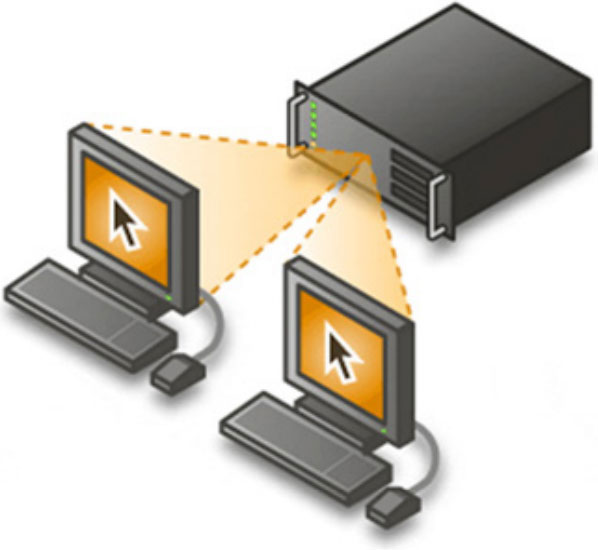
\includegraphics[scale=0.3]{imagens/virtualizacao-apresentacao.jpg}
    	\end{center}
    	\FonteFigura{\citeonline[p. 165]{neto2015ti}.}
    \end{figure}
    
    \item Virtualização de Armazenamento: cria uma camada de abstração entre o sistema operacional e os discos físicos utilizados para armazenamento de dados, permitindo que usuários ou aplicações acessem sem necessidade de informar onde estão localizados ou como é gerenciado (\autoref{fig_virt_arm}).
    
    \begin{figure}[htb]
    	\caption{\label{fig_virt_arm}Virtualização de Armazenamento.}
    	\begin{center}
    	    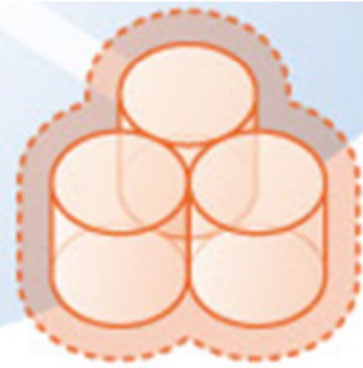
\includegraphics[scale=0.3]{imagens/virtualizacao-armazenamento.jpg}
    	\end{center}
    	\FonteFigura{\citeonline[p. 163]{neto2015ti}.}
    \end{figure}
\end{itemize}

\subsection{Gerenciamento Eletrônico de Documentos}

    
\lipsum[1]
\lipsum[2]
\lipsum[3]

\subsection{Resíduos de Equipamentos Eletroeletrônicos}

Resíduos de Equipamentos Eletroeletrônicos (REEE) é o nome dado a todo resíduo proveniente dos equipamentos eletrônicos \cite[p. 2]{natume2011residuos}. A maioria absoluta desse tipo de resíduo é resultado da obsolescência dos equipamentos eletrônicos, que leva a um descarte de equipamentos antes que esses atinjam seu tempo útil \cite[p. 2]{da2010lixo}. A grande produção de novos aparelhos faz com que os antigos sejam considerados ultrapassados e logo são descartados pelos usuários. Muitas vezes esse descarte é feito de forma inadequada, acarretando assim graves problemas ao meio ambiente.

A \autoref{tab:composicao_fisica} mostra a porcentagem dos principais materiais presentes na composição de um computador, onde eles se encontram e as respectivas porcentagens recicláveis.

\begin{table}[htb]	
    \ABNTEXfontereduzida
	\Caption{\label{tab:composicao_fisica} Composição Física de um computador e índice de materiais recicláveis.}
	\UECEtab{}{
		\begin{tabular}{lp{2.6cm}ll}
			\toprule
    		\textbf{Material} & \textbf{\% em relação ao Peso Total}  & \textbf{\% Reciclável}  & \textbf{Localização} \\
			\midrule \midrule
				Alumínio & 14,172 & 80 & Circuito integrado, solda, bateria \\
				%\midrule
				Chumbo & 6,298 & 5 & Semicondutor \\
				%\midrule
				Ferro & 20,471 & 80 & Estrutura, encaixes \\
				%\midrule
				Estanho & 1,007 & 70 & Circuito integrado \\
				%\midrule
				Cobre & 6,928 & 90 & Condutivo \\
				%\midrule
				Bário & 0,031 & 0 & Válvula eletrônica \\
				%\midrule
				Níquel & 0,850 & 80 & Estrutura, encaixes \\
				%\midrule
				Zinco & 2,204 & 60 & Bateria \\
				%\midrule
				Berílio & 0,015 & 0 & Condutivo térmico, conectores \\
				%\midrule
				Ouro & 0,016 & 98 & Conexão, condutivo \\
				%\midrule
				Manganês & 0,031 & 0 & Estrutura, encaixes \\
				%\midrule
				Prata & 0,018 & 98 & Condutivo \\
				%\midrule
				Cromo & 0,006 & 0 & Decoração, proteção contra corrosão \\
				%\midrule
				Cádmio & 0,009 & 0 & Bateria, chip, semicondutor, estabilizadores \\
				%\midrule
				Mercúrio & 0,002 & 0 & Baterias, ligamentos, termostatos, sensores \\
				%\midrule
				Sílica & 24,880 & 0 & Vidro \\
			\bottomrule
		\end{tabular}
	}{
		\Fonte{\url{http://www.tec.abinee.org.br/2007/arquivos/s702.pdf}}
    }
\end{table}

%pm esse período ficou bem longo também.
%pm vc tá listando três consequências diferentes, dá até pra usar marcador se quiser. enche linguiça e fica menos desgastante de ler
Quando descartados de forma inadequada, em lixões, tem consequências graves ao meio ambiente, como a contaminação de lençóis freáticos e do solo, e às pessoas que entram em contato com esse tipo de lixo devido aos metais pesados neles presentes e as peças plásticas presentes nesses aparelhos demoram cerca de 150 anos para se decompor no meio ambiente \cite[p. 17]{aguilar2009tecnologia}. 

A \autoref{tab:viloes_eletroeletrônicos} mostra os principais metais usados na composição dos equipamentos eletroeletrônicos e os danos causados em humanos que entram em contato com esses equipamentos. Por isso é necessário que o lixo eletrônico seja descartado de forma correta.

\begin{table}[htb]
    \ABNTEXfontereduzida	
	\Caption{\label{tab:viloes_eletroeletrônicos} Os vilões dos eletroeletrônicos.}
	\UECEtab{}{
		\begin{tabular}{p{2cm}p{3.5cm}p{9cm}}
			\toprule
    		\textbf{Substância} & \textbf{Origem} & \textbf{Efeito} \\
			\midrule \midrule
				Mercúrio & Computador, monitor, televisão de tela plana  & Problemas de estômago, distúrbios renais e neurológicos, alterações genéticas e no metabolismo \\
				%\midrule
				Cádmio & Computador, monitor de tubo e baterias & Agente cancerígeno, afeta o sistema nervoso, provoca dores reumáticas, distúrbios metabólicos e 
				problemas pulmonares \\
				%\midrule
				Zinco & Baterias de celulares e laptops & Provoca vômitos, diarreias e problemas pulmonares \\
				%\midrule
				Manganês & Computador e celular & Anemia, dores abdominais, vômito, seborreia, impotência, tremor nas mãos e perturbações emocionais \\
                %\midrule
                Chumbo & Computador, celular e televisão & Irritabilidade, tremores musculares, lentidão de raciocínio, alucinação, insônia e hiperatividade \\
                %\midrule
                PVC & Usado em fios para isolar corrente & Problemas respiratórios  \\
				%\midrule
				Cloreto de Amônia  & Baterias de celulares e laptops & Acumula-se no organismo e provoca asfixia \\
				%\midrule
				Arsênio & Celulares & Agente cancerígeno, afeta o sistema nervoso e cutâneo \\
			\bottomrule
		\end{tabular}
	}{
		\Fonte{Adaptado de \citeonline{moi2014lixo}.}
    }
\end{table}


A melhor forma de evitar a contaminação dos humanos é diminuir a geração desse tipo de resíduo, com a manutenção adequadas dos equipamentos existentes além de práticas que aumentem sua vida útil, bem como destinar os resíduos inevitavelmente gerados para um local específico e adequado para tratamento. Deve haver uma preocupação na produção desses equipamentos, cuidando para que a matéria prima seja bem aproveitada e que não haja desperdícios, além de evitar a produção de equipamentos defeituosos, que terão que ser descartados posteriormente.

A \autoref{fig_percepcao}\footnote{Construído através do Astah Community \url{http://astah.net/editions/community}} apresenta o ciclo de vida de um computador.

\begin{figure}[htb]
	\caption{\label{fig_percepcao}Percepção do problema por mapa conceitual.}
	\begin{center}
	    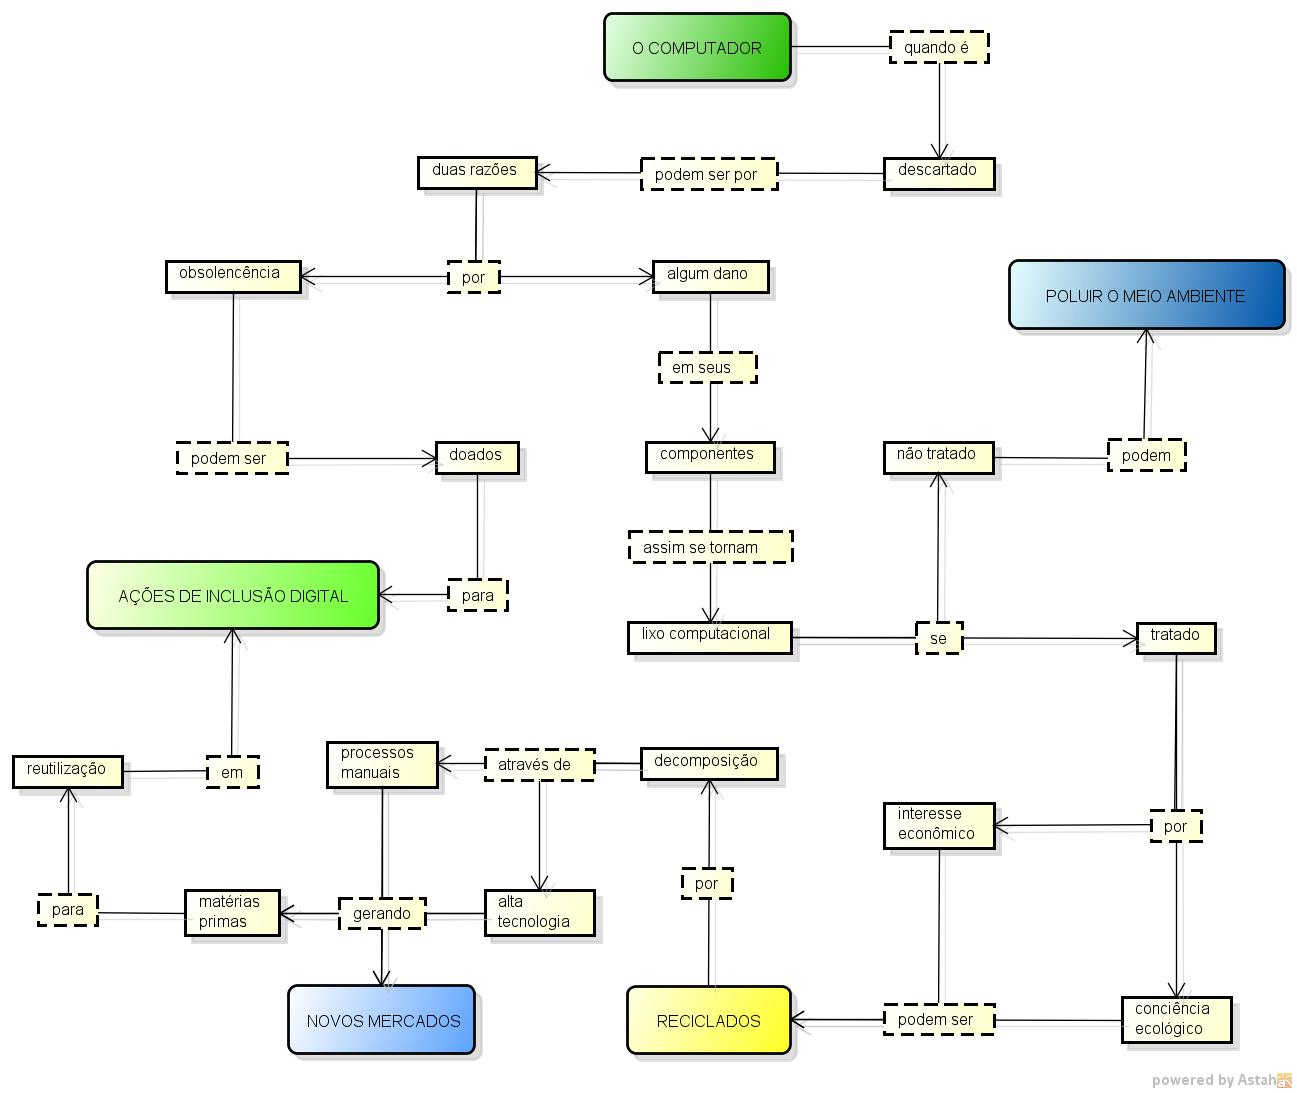
\includegraphics[scale=0.35]{imagens/percepcao-problema.jpg}
	\end{center}
	\Fonte{\citeonline[p. 263]{calvao2009lixo} (Adaptado pelo autor).}
\end{figure}

\subsection{Os cinco R's da educação ambiental}

Os cinco R’s da educação ambiental correspondem a práticas que podem ser implantadas em qualquer lugar e tem impacto que não se limitam ao local em que são aplicados. Sua implantação gera uma economia de recursos elétricas, hídricos e de matéria-prima em geral, além de contribuir para a maior vida útil dos produtos. Como postos nos trabalhos de CITAR os cinco R's podem ser definidos da seguinte forma:

\subsubsection{Repensar}
Antes de adquirir um produto ou serviço deve-se refletir sobre sua real necessidade, ponderando o seu benefício e o impacto ambiental por ele gerado. Além disso deve-se pensar na sua vida útil e em seu posterior descarte, em como ele deve ser feito de forma adequada.

\subsubsection{Recusar}
Caso o produto de interesse não seja de fato necessário, deve-se recusá-lo. Essa prática se aplica a produtos e serviços oferecidos, vide a prática de repensar para decidir sobre sua aceitação ou recusa. Essa prática é muito relevante frente a produtos que contenham materiais que agridam ao meio ambiente e sejam de difícil reciclagem ou demorem para se decompor.

\subsubsection{Reduzir}
Corresponde à redução no consumo de produtos e serviços em geral. Além de reduzir também os gastos que eles geram, desligando aparelhos eletroeletrônicos quando esses não forem usados. Aqui entra também a preferência por produtos de maior durabilidade e que ofereçam menor potencial de geração de resíduos. Isso impacta na redução no número de produtos consumidos e redução nos resíduos gerados.

\subsubsection{Reutilização}
A reutilização corresponde ao uso repetido de um produto, seja para a mesma finalidade sempre, ou dando outra utilidade para ele. Além da troca e doação de produtos para outras pessoas ou empresas.

\subsubsection{Reciclar}
A reciclagem contribui para a economia de recursos usados na produção e no tratamento de resíduos, além de contribuir para a não contaminação de solos e até pessoas pelo descarte inadequado. O ideal é que haja uma separação conforme o tipo de materiais presentes nos resíduos antes da entrega nos postos de coleta seletiva. Essa prática contribui gerando emprego e renda para as pessoas envolvidas, além de resíduos gerados.


\section{Normas, Regulamentações e Certificados}
%pm joga o link do pdf em scholar.google.com
%pm exporta pra bibtex e cola no seu referencias
%pm /cite{nome} e já é
Existem Normas e certificações que servem para regulamentar e atestar as práticas de TI Verde internacional e nacionalmente. Alguns exemplos de certificações internacionais são: ISO 14001, RoHS e Selo Verde, etc. Essas certificações se referem ao processo de trabalho da TI, tanto para a fabricação, quanto para o uso de equipamentos eletrônicos. (Fonte artigo https://assets.itpac.br/arquivos/Revista/42/3.pdf)

\subsection{ISO 14001}
%pm joga o link do pdf em scholar.google.com
%pm exporta pra bibtex e cola no seu referencias
%pm /cite{nome} e já é
A ISO 14001 corresponde a normas que regulamentam os padrões de práticas do trabalho de organizações públicas ou privadas que buscam realizar suas atividades de forma sustentável visando produzir produtos de qualidade que sejam ecologicamente corretos. Fonte artigo https://assets.itpac.br/arquivos/Revista/42/3.pdf

A implantação dessas práticas leva uma revisão dos processos da organização certificada, o que contribui para a redução de poluição, seja pelo lançamentos de gases à atmosfera ou pelos resíduos gerados. 


%A ABNT NBR ISO 14001 é uma norma aceita internacionalmente que define os requisitos para colocar um sistema da gestão ambiental em vigor. Ela ajuda a melhorar o desempenho das empresas por meio da utilização eficiente dos recursos e da redução da quantidade de resíduos, ganhando assim vantagem competitiva e a confiança das partes interessadas.

%A ABNT NBR ISO 14001 adequa-se a todos os tipos e tamanhos da empresa. Ela exige que as empresas considerem todas as questões ambientais relativas às suas operações, como a poluição do ar, questões referentes à água e ao esgoto, a gestão de resíduos, a contaminação do solo, a mitigação e adaptação às alterações climáticas e a utilização e eficiência dos recursos.

%Assim como todas as normas de sistemas da gestão, a ABNT NBR ISO 14001 inclui a necessidade de melhoria contínua dos sistemas de uma empresa e a abordagem de questões ambientais. A norma foi recentemente revista, com melhorias fundamentais, como o aumento da crescente relevância da gestão ambiental nos processos de planejamento estratégico da empresa, maior contribuição por parte da liderança e um compromisso intenso em relação a iniciativas proativas que impulsionem o desempenho ambiental.

%pm usa os marcador certo aqui
%Existem inúmeros motivos para as empresas adotarem uma abordagem estratégica a fim de melhorar o seu desempenho ambiental. Os usuários da norma relataram que a ABNT NBR ISO 14001 ajuda a: • Demonstrar conformidade com requisitos legais e regulamentares atuais e futuros • Aumentar o envolvimento da liderança e o comprometimento dos funcionários • Melhorar a reputação da empresa e a confiança das partes interessadas mediante comunicação estratégica • Alcançar os objetivos estratégicos de negócios através da incorporação de questões ambientais na gestão das empresas. • Oferecer vantagem competitiva e financeira aumentando a eficiência e reduzindo custos • Incentivar a melhoria do desempenho ambiental por parte de fornecedores, integrando-os aos sistemas de negócios da empresa

%A ABNTNBR ISO 14001:2015 passa a exigir: • Que a gestão ambiental seja mais importante no posicionamento estratégico da empresa • Maior comprometimento da liderança • A implementação de iniciativas proativas que visem proteger o meio ambiente contra danos e degradação, como por exemplo, o uso sustentável dos recursos e a mitigação das alterações climáticas • Enfoque no conceito de ciclo de vida a fim de garantir que aspectos ambientais sejam levados em consideração desde o desenvolvimento até o fim da vida útil do produto • A adoção de uma estratégia de comunicação com foco nas partes interessadas Além disso, ela possibilita uma integração mais fácil a outros sistemas de gestão, visto que têm a mesma estrutura e os mesmos termos e definições.
    

\subsection{RoHS}

%pm adiciona isso na lista de siglas, não?
O RoHS (Restriction of Certain Hazardous Substances) ou Restrição de Certas Substâncias Perigosas, também conhecida como a Lei do Sem Chumbo (lead-free), foi criada em julho de 2006 na União Européia. Essa foi uma das primeiras leis a pressionarem as fabricantes de TI. Após a criação da RoHS, as empresas, industrias e importadores também tem o objetivo de se responsabilizar pelo “ciclo de vida” dos produtos que insere no mercado de consumo. Fonte monografia

Entretanto existe uma teoria, do reciclável poluidor, que trata a reciclagem desse REEE como algo tão poluente como o descarte em aterros, bem como a teoria da diminuição do ciclo de vida dos componentes eletrônicos, uma vez que a reciclagem dos componentes pode dar origem a produtos com curta vida útil (Garcia e Milagre, 2008). 

\subsection{WEEE}

A WEEE (Waste Electrical and Electronic Equipment Directive) ou Diretiva para o Lixo Elétrico e Equipamentos Eletrônicos também foi criada na Europa com o objetivo de preservar a natureza, essa diretiva determina como compromisso dos fabricantes o recolhimento e a destinação correta dos resíduos por eles gerados. A WEEE também prevê a reciclagem, recuperação e reutilização dos resíduos para que estes sejam reduzidos \cite{neto2015ti}.

\subsection{Selo Verde}

O selo verde é uma forma de reconhecimento de espaços, produtos e serviços que contribuam para a preservação ambiental. Tal selo é atribuído as organizações depois das organizações passarem por controle de qualidade ambiental. Com isso há o incentivo a promoção de soluções ambientais (Fonte: http://seloverde.org/), uma vez que os critérios utilizados para certificar uma organização são:  a promoção da conscientização ambiental na comunidade que adquire seus produtos ou serviços, ser economicamente viável e promover a sustentabilidade econômica do ambiente digital e ser ambientalmente responsável, aplicando os 5R’s em seus processos de forma a produzir com economia de energia ou com pequena quantidade de substâncias tóxicas. (Fonte: implementacoa de praticas sustentaveis em empresas.pdf). 
É uma forma de incentivar as empresas a fabricarem produtos com baixa quantidade de produtos químicos (Fonte: https://assets.itpac.br/arquivos/Revista/42/3.pdf), além de ser um diferencial no mercado. Alguns dos órgãos responsáveis pela aplicação desses selos são: o Greenpeace, o Centro de Computação Eletrônica da Universidade de São Paulo, Instituto da Qualidade Automotiva e Forset Stewardship Council- FSC.  (Fonte: https://assets.itpac.br/arquivos/Revista/42/3.pdf)


\subsection{Energy Star}

Energy Star e um programa da U.S. Environmental Protection Agency(EPA) que incentiva a redução na quantidade de energia consumida as organizações. Uma de suas práticas é oferecer selos aos fabricantes de equipamentos eletrônicos que optarem pela utilização de tecnologias com funções para poupar energia.

\subsection{Procel}

O Selo Procel de Economia de Energia foi criado pelo Programa Nacional de Conservação de Energia Elétrica – Procel, programa instituído por Decreto Presidencial em 8 de dezembro de 1993, sendo desde então executado pela Eletrobras. O objetivo é criar uma identificação para que o consumidor conheça os equipamentos e eletrodomésticos mais eficientes e que consomem menos energia.

A classificação dos equipamentos é feita de acordo com os índices de consumo e desempenho estabelecidos para cada categoria de equipamento. Para receber o selo cada equipamento é submetido a ensaios em laboratórios indicados pela Eletrobras.


\subsection{Legislação Brasileira}
%pm Lei não é publicação científica.
%pm essas porra vira tudo footnote, com a \url de cada uma e a data de acesso.

Lei nº 12.305 de 2 de agosto de 2010. (projeto de lei 2061/07)

No Brasil, a Lei nº 12.305, de 02 de agosto de 2010, institui a Política Nacional de Resíduos Sólidos, dispõe “sobre seus princípios, objetivos e instrumentos, bem como sobre as diretrizes relativas à gestão integrada e ao gerenciamento de resíduos sólidos, incluídos os perigosos, às responsabilidades dos geradores e do poder público e aos instrumentos econômicos aplicáveis. ” (LEI Nº 12.305, 2010, Art. 1o  § 1º, p. 1).

Alguns princípios e objetivos da Política Nacional de Resíduos Sólidos são: o desenvolvimento sustentável; a ecoeficiência, visando fornecimento de bens e serviços de um melhor custo-benefício e redução de impactos ambientais; a responsabilidade compartilhada pelo ciclo de vida dos produtos; a proteção da saúde pública e da qualidade ambiental; a aplicação de alguns dos 5R’s, bem como o tratamento adequada dos rejeitos. (Lei Nº 12.305, 2010, Art. 6º e 7º)

No que diz respeito a tecnologia da informação, um dos objetivos trata da “adoção, desenvolvimento e aprimoramento de tecnologias limpas como forma de minimizar impactos ambientais (Art. 7o IV).

Uma das diretrizes trata da ordem de prioridade na gestão e gerenciamento de resíduos sólidos: “não geração, redução, reutilização, reciclagem, tratamento dos resíduos sólidos e disposição final ambientalmente adequada dos rejeitos.” (Art. 9o)

Os responsáveis pelo destino dos resíduos de eletrônicos são definidos no Art. 33. São eles os fabricantes, importadores, distribuidores e comerciantes de produtos eletroeletrônicos. Eles tem como obrigação “a estruturar e implementar sistemas de logística reversa, mediante retorno dos produtos após o uso pelo consumidor, de forma independente do serviço público de limpeza urbana e de manejo dos resíduos sólidos”. Além disso devem “tomar todas as medidas necessárias para assegurar a implementação e operacionalização do sistema de logística reversa sob seu encargo [...], podendo, [...] implantar procedimentos de compra de produtos ou embalagens usados; disponibilizar postos de entrega de resíduos reutilizáveis e recicláveis; atuar em parceria com cooperativas ou outras formas de associação de catadores de materiais reutilizáveis e recicláveis” (Art. 33. § 3o I, II e III).

O Art. 5o diz que a “Política Nacional de Resíduos Sólidos integra a Política Nacional do Meio Ambiente e articula-se com a Política Nacional de Educação Ambiental, regulada pela Lei no 9.795, de 27 de abril de 1999, com a Política Federal de Saneamento Básico, regulada pela Lei nº 11.445, de 2007. Além delas se aplica também aos resíduos sólidos a lei nos 11.445, de 5 de janeiro de 2007, dentre outras normas (Art. 2o).

Política Nacional de Educação Ambiental (Lei nº 9.785 de 27 de abril de 1999). 

Nessa lei a educação ambiental é tratada como “os processos por meio dos quais o indivíduo e a coletividade constroem valores sociais, conhecimentos, habilidades, atitudes e competências voltadas para a conservação do meio ambiente, bem de uso comum do povo, essencial à sadia qualidade de vida e sua sustentabilidade. (Art. 1o)

Segunda Art. 2o da Lei, cabe às empresas, entidades de classe, instituições públicas e privadas, a promoção de “programas destinados à capacitação dos trabalhadores, visando à melhoria e ao controle efetivo sobre o ambiente de trabalho, bem como sobre as repercussões do processo produtivo no meio ambiente”. Além disso, empresas públicas e privadas devem ser incentivadas, pelo Poder Público, em níveis federal, estadual e municipal, a participarem do desenvolvimento de programas de educação ambiental (Art. 13. Parágrafo único III) não formal, que tem por objetivo sensibilizar a população em geral sobre as questões ambientais e à sua organização e participação na defesa da qualidade do meio ambiente. (Art. 13.)

Política Federal de Saneamento Básico (Lei nº 11.445 de 2007)

Um dos princípios fundamentais dessa lei é a “utilização de tecnologias apropriadas [...] e a adoção de soluções graduais e progressivas (Art. 2o  VIII) e uma das diretrizes incentiva o “desenvolvimento científico e tecnológico, à adoção de tecnologias apropriadas e à difusão dos conhecimentos gerados” (Art. 48. VIII). Essa lei também estimula o “uso de tecnologias modernas e eficientes, compatíveis com os níveis exigidos de qualidade, continuidade e segurança na prestação dos serviços” (Art. 29.  § 1o  VII).

% ----------------------------------------------------------
% PARTE III
% ----------------------------------------------------------
\part{Levantamento amostral}

% ----------------------------------------------------------
% PARTE III
% ----------------------------------------------------------
\part{Resultados}

% ----------------------------------------------------------
% Finaliza a parte no bookmark do PDF para que se inicie o bookmark na raiz e adiciona espaço de parte no Sumário
% ----------------------------------------------------------
\phantompart


% ----------------------------------------------------------
% ELEMENTOS PÓS-TEXTUAIS
% ----------------------------------------------------------
\postextual

% Referências bibliográficas
\bibliography{bibtex/referencias}

% Apêndices
%% Apêndices
% ---
% Inicia os apêndices
% ---
\begin{apendicesenv}

% Imprime uma página indicando o início dos apêndices
\partapendices

% ----------------------------------------------------------
\chapter{Quisque libero justo}
% ----------------------------------------------------------

\lipsum[50]

% ----------------------------------------------------------
\chapter{Nullam elementum urna vel imperdiet sodales elit ipsum pharetra ligula
ac pretium ante justo a nulla curabitur tristique arcu eu metus}
% ----------------------------------------------------------
\lipsum[55-57]

\end{apendicesenv}
% ---


% Anexos
%% ----------------------------------------------------------
% Anexos
% ---
% Inicia os anexos
% ---
\begin{anexosenv}

% Imprime uma página indicando o início dos anexos
\partanexos

% ---
\chapter{Morbi ultrices rutrum lorem.}
% ---
\lipsum[30]

% ---
\chapter{Cras non urna sed feugiat cum sociis natoque penatibus et magnis dis
parturient montes nascetur ridiculus mus}
% ---

\lipsum[31]

% ---
\chapter{Fusce facilisis lacinia dui}
% ---

\lipsum[32]

\end{anexosenv}


%---------------------------------------------------------------------
% INDICE REMISSIVO
%---------------------------------------------------------------------
\phantompart
\printindex
%---------------------------------------------------------------------

\end{document}
